\section{Dataset and Benchmark Details}
\label{app:dataset}

\subsection{Simulation}
\paragraph{Training}
Table~\ref{tab:mixture} summarizes the Open-X-Embodiment dataset we use for the base model CogACT \cite{li2024cogact}. Table~\ref{tab:libero-data} summarizes the LIBERO dataset we use for the base model OpenVLA-OFT~\cite{kim2025fine}.

\begin{table}[htbp]
\centering
    \caption{Open-X-Embodiment dataset composition we use for CogACT training.}
    \label{tab:mixture}
    \begin{tabular}{lr}
    \toprule
     Dataset & Ratio \\
    \midrule
     Fractal~\citep{brohan2022rt} & 27.1\% \\
     Kuka~\citep{kalashnikov2018scalable} & 14.7\% \\
     Bridge~\citep{walke2023bridgedata,Ebert2021BridgeDB} & 15.3\% \\
     Taco Play~\citep{rosete2023latent,mees2023grounding} & 3.4\% \\
     Jaco Play~\citep{dass2023jacoplay} & 0.6\% \\
     Berkeley Cable Routing~\citep{luo2024multi} & 0.3\% \\
     Roboturk~\citep{mandlekar2018roboturk} & 2.7\% \\
     Viola~\citep{zhu2023viola} & 1.1\% \\
     Berkeley Autolab UR5~\citep{BerkeleyUR5Website} & 1.4\% \\
     Toto~\citep{zhou2023train} & 2.3\% \\
     Stanford Hydra Dataset~\citep{belkhale2023hydra} & 5.1\% \\
     Austin Buds Dataset~\citep{zhu2022bottom} & 0.2\% \\
     NYU Franka Play Dataset~\citep{cuiplay} & 1.0\% \\
     UCSD Kitchen Dataset~\citep{ucsdkitchens} & $<$0.1\% \\
     Austin Sailor Dataset~\citep{nasiriany2023learning} & 2.5\% \\
     Austin Sirius Dataset~\citep{liu2022robot} & 2.0\% \\
     DLR EDAN Shared Control~\citep{quere2020shared} & $<$0.1\% \\
     IAMLab CMU Pickup Insert~\citep{saxena2023multi} & 1.0\% \\
     UTAustin Mutex~\citep{shahmutex} & 2.6\% \\
     Berkeley Fanuc Manipulation~\citep{zhu2023fanuc} & 0.9\% \\
     CMU Stretch~\citep{mendoncastructured} & 0.2\% \\
     BC-Z~\citep{jang2022bc} & 8.6\% \\
     FMB Dataset~\citep{luo2023fmb} & 2.4\% \\
    \bottomrule
    \end{tabular}
\end{table}

\begin{table}[htbp]
    \caption{LIBERO dataset}
    \label{tab:libero-data}
    \centering
    \begin{tabular}{c|cccc}
    \toprule
         Dataset & Libero-Spatial & Libero-Object & Libero-Goal & Libero-Long \\
    \midrule
       \#(trajectories) & 432 & 454 & 428 & 379 \\
    \bottomrule
    \end{tabular}

\end{table}

\paragraph{SimplerEnv} SimplerEnv \cite{li2024evaluating} is a simulation-based benchmark designed for tabletop robotic manipulation. It is explicitly constructed to minimize the sim-to-real gap, demonstrating strong alignment between simulation performance and real-world execution across multiple robot platforms. The benchmark supports two complementary evaluation configurations: Visual Matching, which emphasizes high visual fidelity to real-world environments, and Variant Aggregations, which systematically introduce visual perturbations such as changes in background, lighting, distractors, and surface textures to assess robustness. SIMPLER includes tasks instantiated on both the Google Robot and the WidowX robot, covering a diverse set of manipulation primitives such as picking, placing, navigation, and articulated object interaction. In all tasks, agents receive RGB visual observations and natural language instructions. SIMPLER offers two evaluation settings:
\begin{itemize}[noitemsep,topsep=0pt,leftmargin=*]
    \item \emph{Visual Matching:} Real-world images are overlaid onto simulated environments, with foreground objects and robots adjusted to closely match real-world appearances.
    \item \emph{Variant Aggregation:} Multiple environmental variations are generated—such as different backgrounds, lighting conditions, and surface textures.
\end{itemize}

\paragraph{LIBERO} LIBERO is built around a simulated Franka Emika Panda arm and provides high-quality human-teleoperated demonstration data paired with language-conditioned tasks to support sample-efficient learning and generalization. The benchmark comprises four distinct task suites—LIBERO-Spatial, LIBERO-Object, LIBERO-Goal, and LIBERO-Long, each providing 10 distinct tasks.


\subsection{Real-World}
\label{app:real}

\begin{figure}
    \centering
    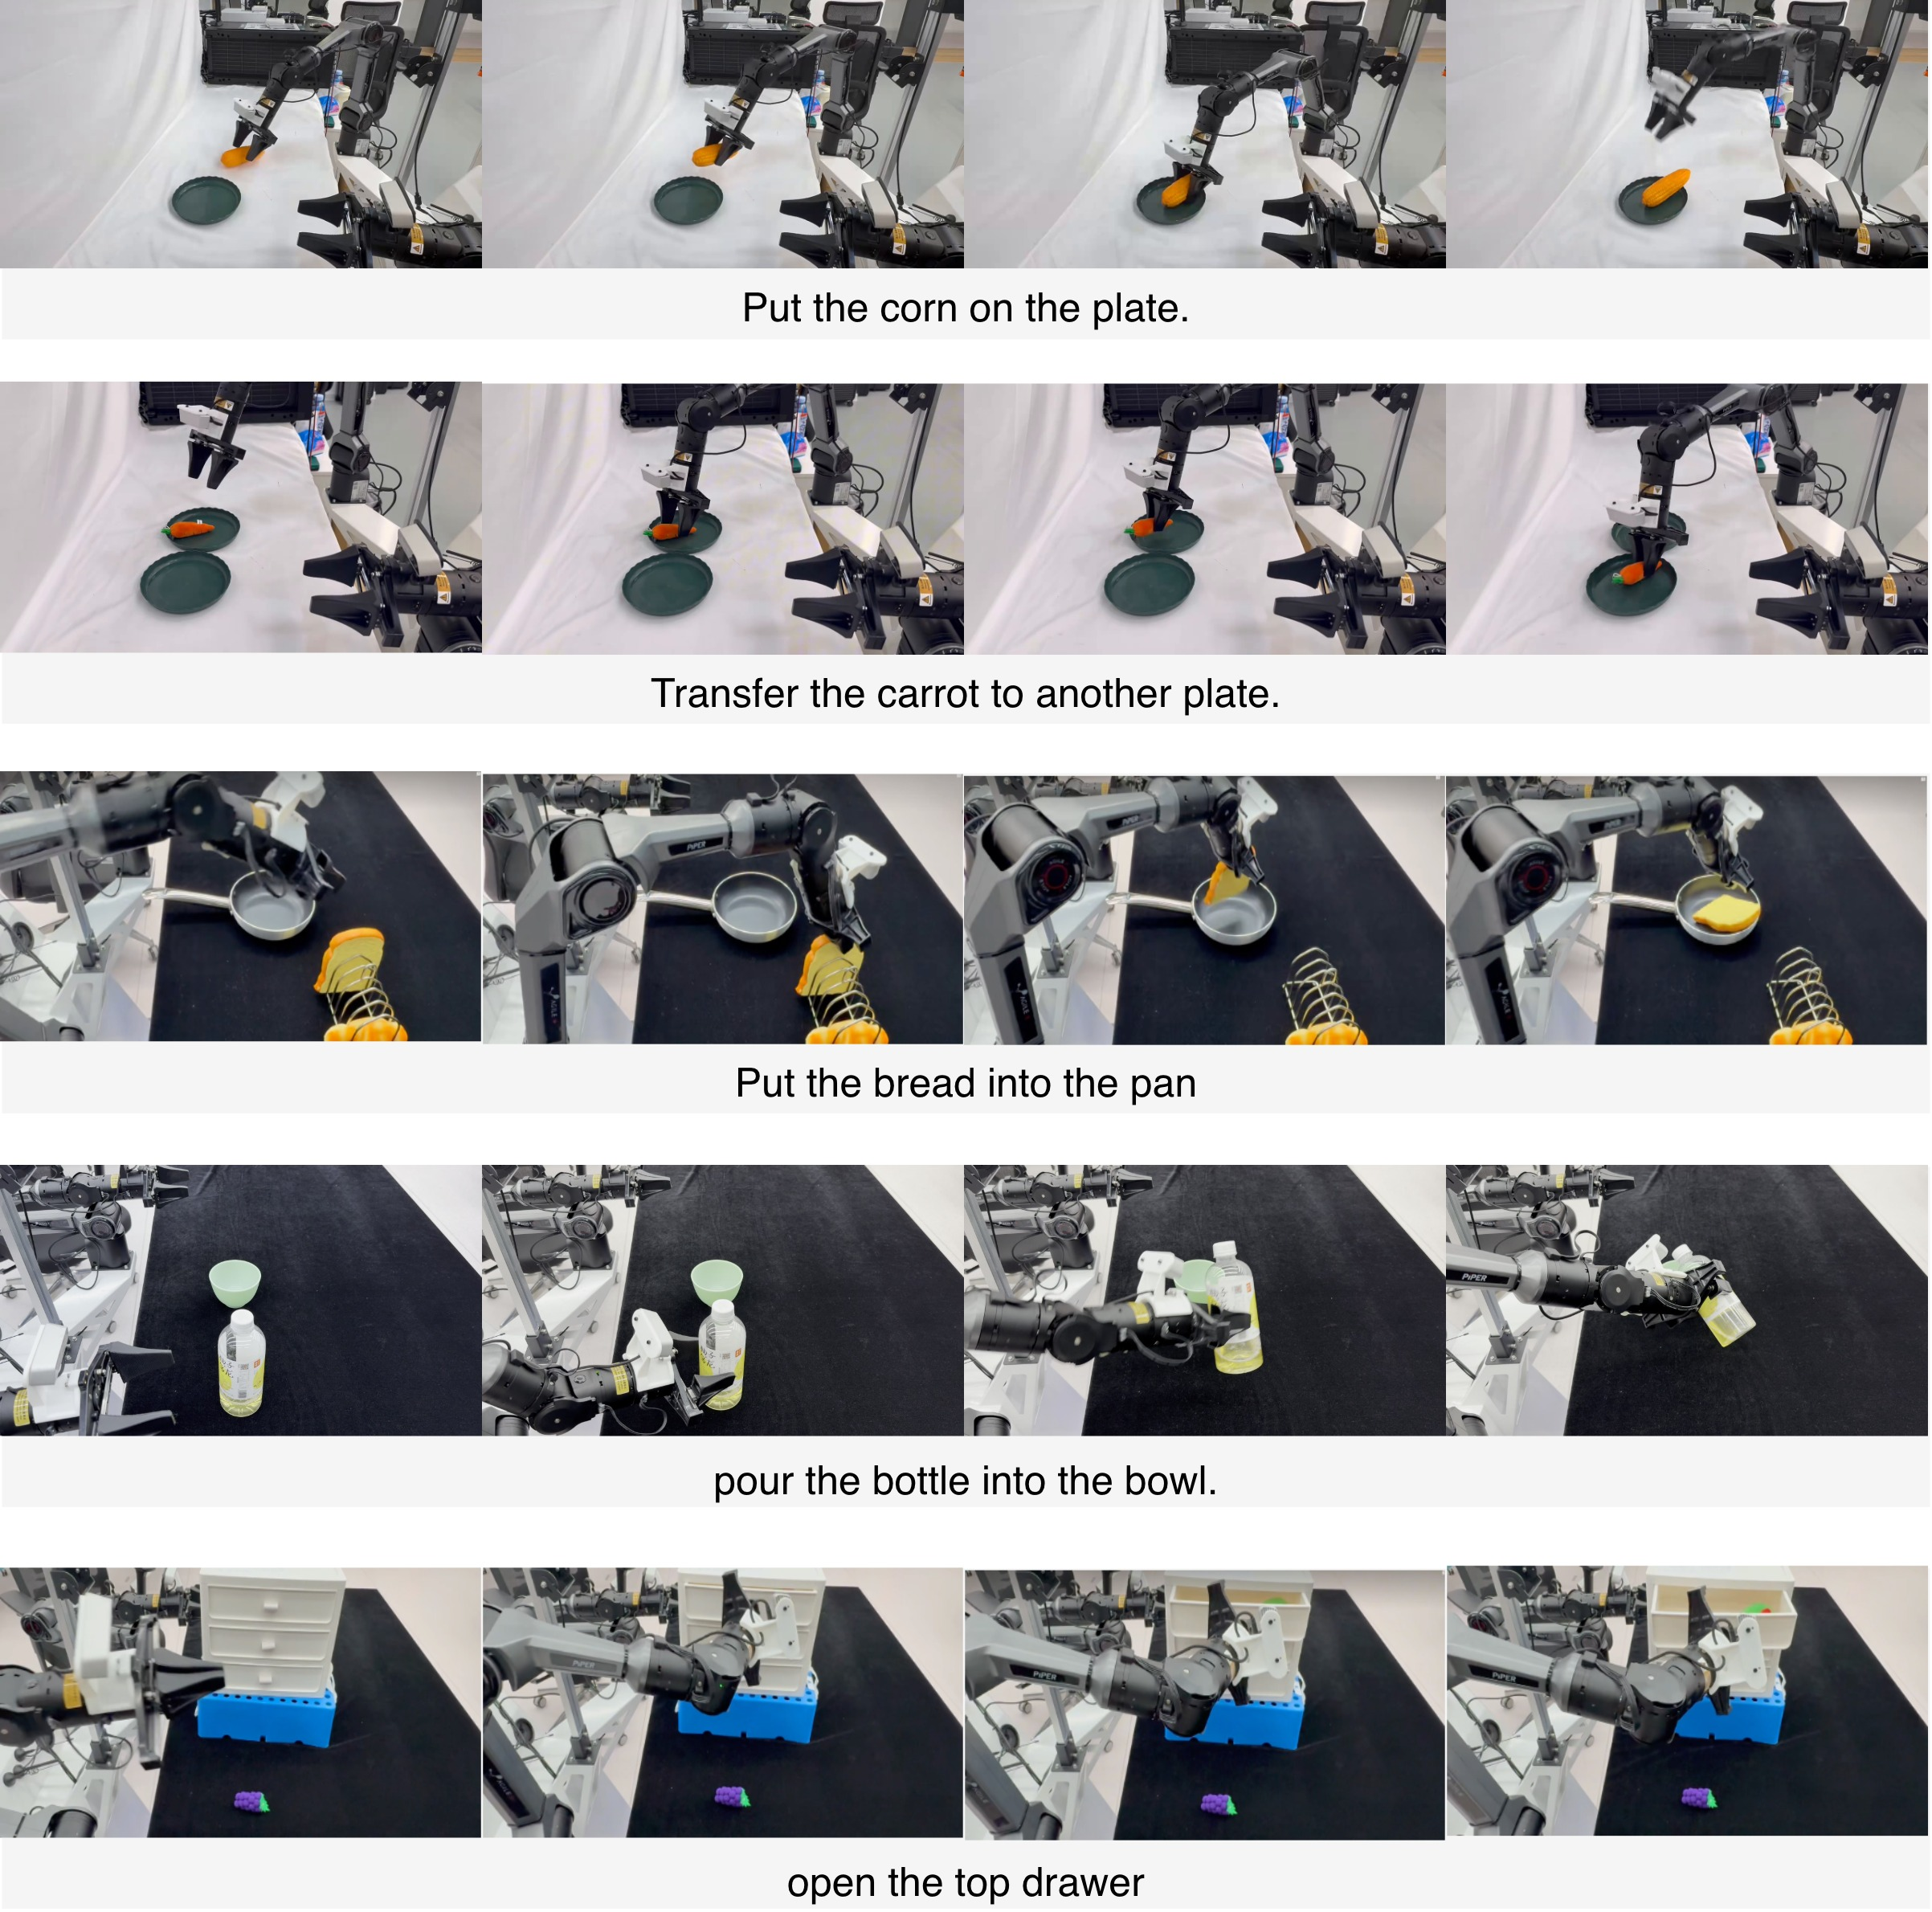
\includegraphics[width=\linewidth]{figs/real_demo.jpg}
    \caption{In real-world evaluations with the Cobot Magic robot, each task is evaluated over 20 episodes.}
    \label{fig:real}
\end{figure}
For the acceleration experiments, we include 7 tasks across 3 categories in the acceleration experiment, with 20 episodes used for training and 20 trials used for evaluating each task. The task designs are detailed below:
\begin{itemize}
\item \textbf{Pick-and-Place.} The robot is instructed to move an object from its original location to a specified destination (e.g., a pan or pot). We report the success rate for each object.
\item \textbf{Pouring.} The robot is instructed to pour the contents of a bottle or can into a container. We report the success rate for each target container.
\item \textbf{Drawer Opening.} The robot is instructed to open a specified drawer. We report the success rate of successfully opening the drawer.
\end{itemize}

For each task, we vary both the object's location and the robotic arm's starting position. The demonstrations of tasks are illustrated in Figure~\ref{fig:real}.

\section{Architecture Details}
\label{app:arch}

\paragraph{Recache gate}
The recache gate is designed to predict the probability of refreshing cached representations based on images (or their latent representations) observed at different timesteps. To minimize additional inference latency in the VLA, the recache gate must remain lightweight. Accordingly, we adopt a simple MLP-based architecture.

As illustrated in Figure~\ref{fig:cache_gate}, the gate takes as input latent embeddings $\bs{Z}_{t_1}$ and $\bs{Z}_{t_2}$ produced by the VLA’s vision backbone at two different timesteps. We first apply a position-wise feedforward network to each embedding. The embeddings are then transposed to enable a channel-wise feedforward operation. After these transformations and dimensionality reduction, the resulting features are flattened and passed through a final MLP to predict the recache probability. For different static levels, we share all parameters except for the final prediction head.

\begin{figure}
    \centering
    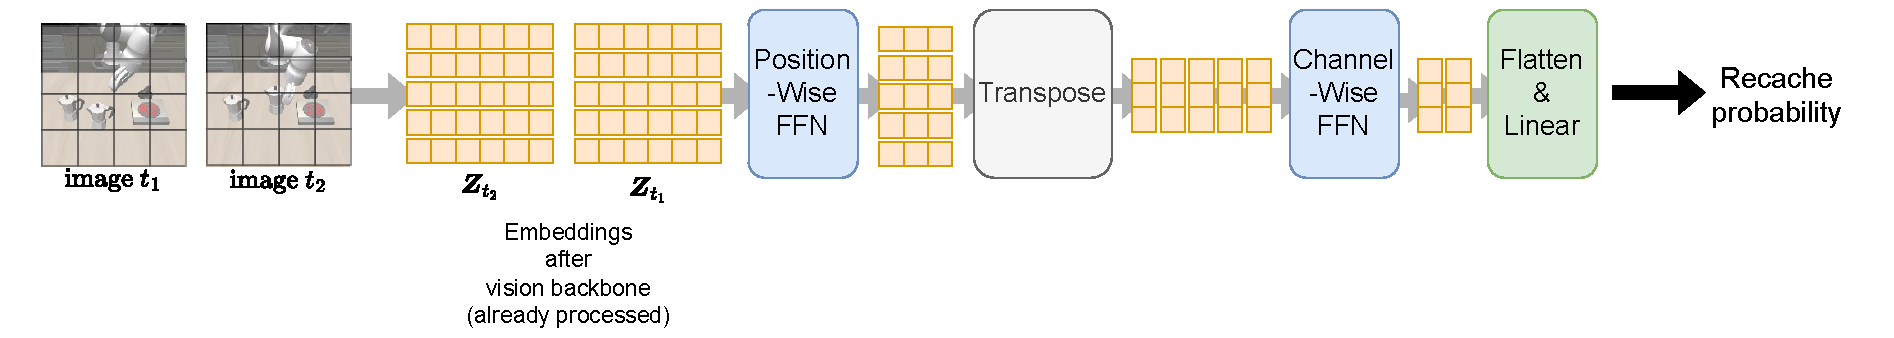
\includegraphics[width=\linewidth]{figs/cache_gate.pdf}
    \caption{Architecture of the recache gate.}
    \label{fig:cache_gate}
\end{figure}


\section{LIBERO-Memory Benchmark}
\label{app:dataset_memory}
Following the LIBERO benchmark \cite{liu2023libero}, the layout initialization is specified by the BDDL scene description file, which is a file format that specifies the initial layout's sampling strategy and other meta information.


\begin{lstlisting}[language=PDDL, caption=An example of the PDDL scene description file used in LIBERO-Memory.]
(define (problem LIBERO_Kitchen_Tabletop_Manipulation)
  (:domain robosuite)
  (:language Heat the tomato sauce on the stove for 1.4 second and then heat the alphabet soup)
    (:regions
      (operation_region
          (:target kitchen_table)
          (:ranges (
              (-0.2 0.09999999999999999 0.0 0.2)
            )
          )
          (:yaw_rotation (
              (0.0 0.0)
            )
          )
      )
      (stove_region
          (:target kitchen_table)
          (:ranges (
              (-0.30000000000000004 -0.2 -0.1 -0.09999999999999999)
            )
          )
          (:yaw_rotation (
              (0.0 0.0)
            )
          )
      )
      (cook_region
          (:target flat_stove_1)
      )
    )

  (:fixtures
    kitchen_table - kitchen_table
    flat_stove_1 - flat_stove
  )

  (:objects
    alphabet_soup_1 - alphabet_soup
    tomato_sauce_1 - tomato_sauce
  )

  (:obj_of_interest
    tomato_sauce_1
    alphabet_soup_1
  )

  (:init
    (On tomato_sauce_1 kitchen_table_operation_region)
    (On alphabet_soup_1 kitchen_table_operation_region)
    (On flat_stove_1 kitchen_table_stove_region)
    (Turnon flat_stove_1)
  )

  (:goal
    (And (CloseXY tomato_sauce_1) (On alphabet_soup_1 flat_stove_1_cook_region))
  )

)
\end{lstlisting}

\paragraph{Oracle demonstrations}
We generate expert trajectories programmatically because the correct behavior in LIBERO-Memory is fully specified and unambiguous. For example, for a sub-task such as “place the tomato sauce can on the stove”, an oracle with access to the simulator state can deterministically execute the correct sequence. The oracle knows the target object and its current location, and issues movement commands that drive the end-effector toward that location. After each movement, it compares the updated end-effector position with the desired target and decides the next control direction. Once the end-effector is sufficiently close, the oracle closes the gripper to grasp the object and subsequently moves it to the specified target location.

Figure~\ref{fig:memory_examples} shows more detailed example trajectories of the benchmark. Figure~\ref{fig:stats} shows the distribution of the trajectory length of the benchmark.

 To better contextualize the absolute performance of our model, we include a human baseline for the benchmark in Table~\ref{tab:stove_human}. Specifically, we recruited two human participants familiar with the task setup, who performed the tasks using standard keyboard controls. Each human participant completed 50 rollout episodes. The performance varies across subtasks: \emph{On Stove} is largely semantic and can be solved reliably by humans, while \emph{Position Reset} and \emph{Doneness} require precise tracking of spatial locations and elapsed time over long horizons, making them more challenging for humans and highlighting greater potential for machine learning models to excel.

\begin{figure}
    \centering
    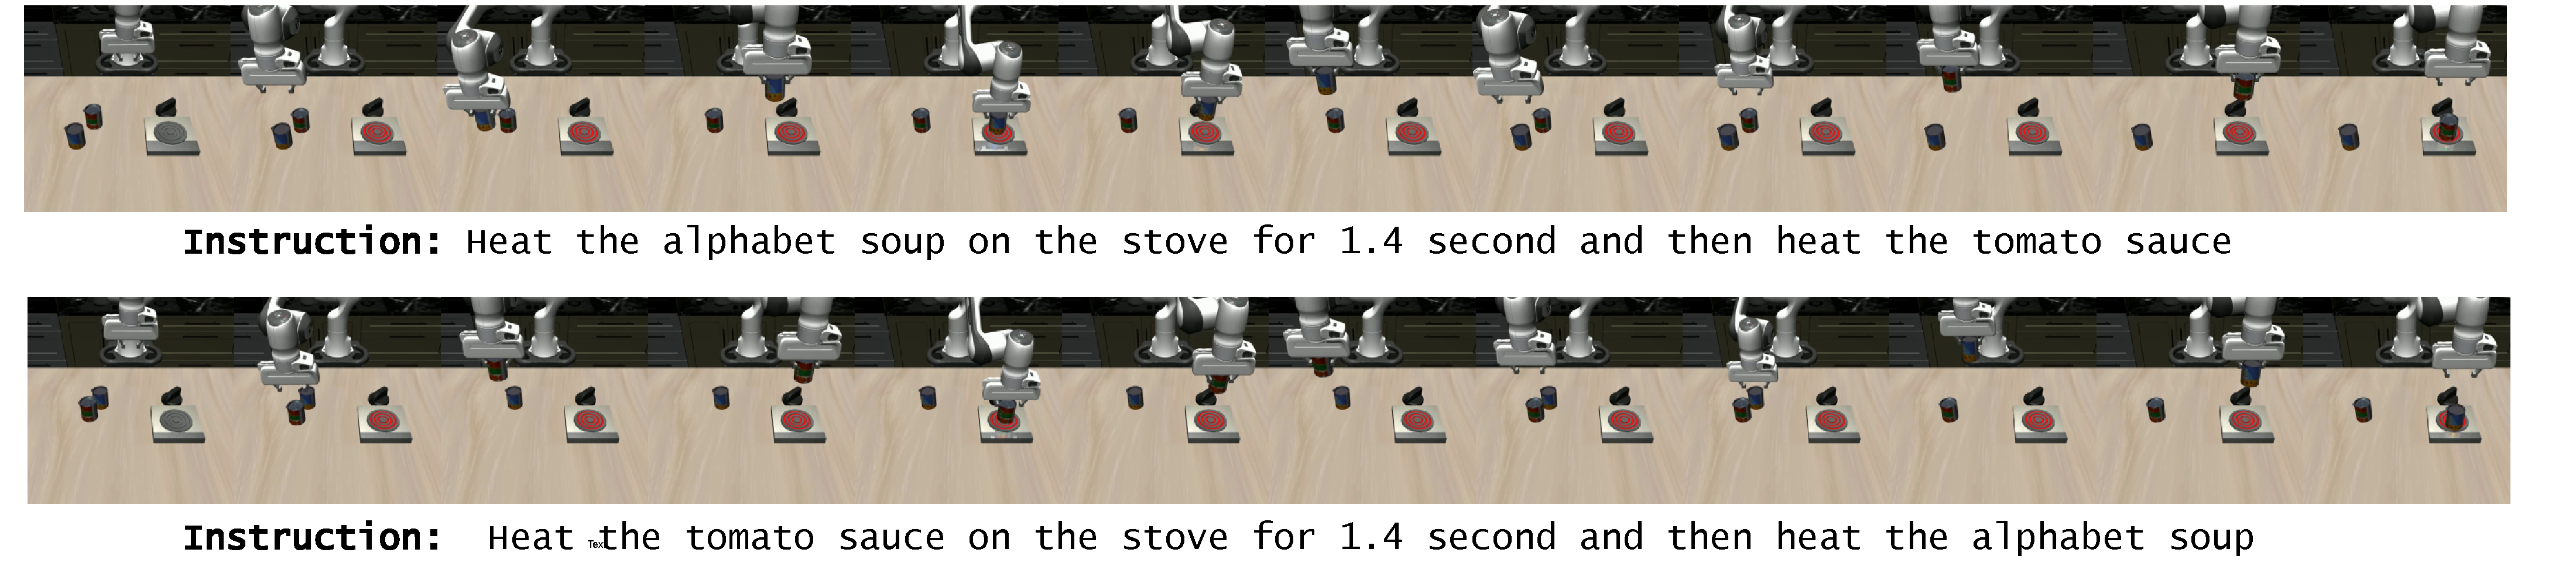
\includegraphics[width=\linewidth]{figs/memory_examples.pdf}
    \caption{Examples of our proposed LIBERO Memory Benchmark.}
    \label{fig:memory_examples}
\end{figure}

\begin{figure}
    \centering
    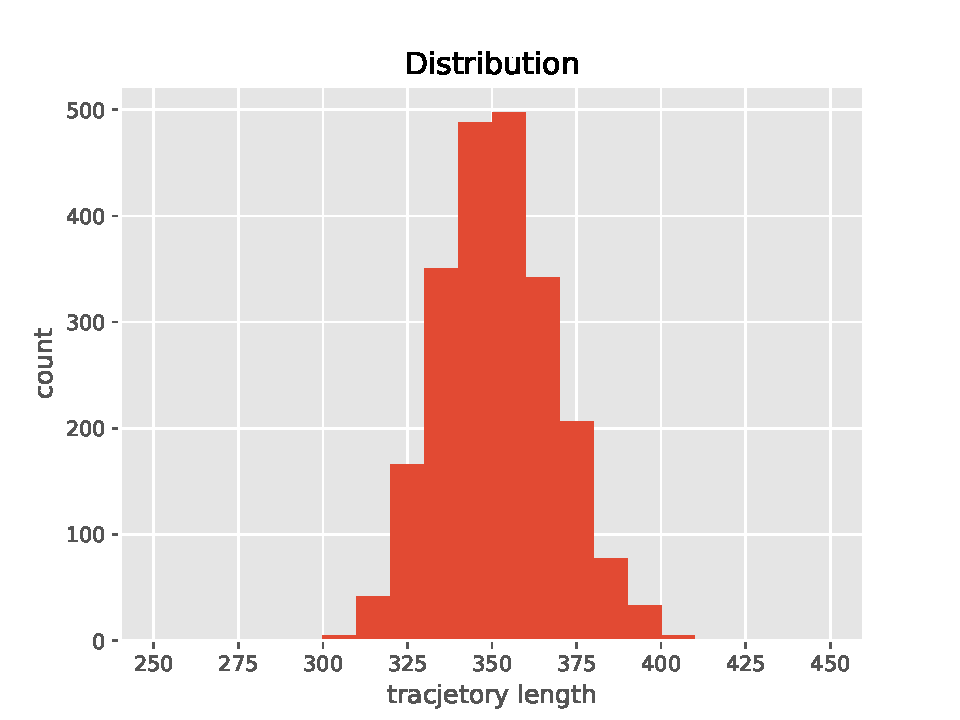
\includegraphics[width=0.5\linewidth]{figs/stats.pdf}
    \caption{Distribution of the trajectory length of the LIBERO-Memory benchmark}
    \label{fig:stats}
\end{figure}

\begin{table}[H]
    \centering
    \caption{Human Performance on LIBERO-Memory.}
    \label{tab:stove_human}
    % \resizebox{\linewidth}{!}{
    \begin{tabular}{lccc}
    \toprule
        Models & On Stove $\uparrow$ & Position Reset $\uparrow$ & Doneness $\downarrow$ \\
    \midrule
    Human 1 & $98.0\%$  & $74.0\%$ & $1.58$ \\
        Human 2 & $96.0\%$ & $68.0\%$ & $1.44$\\
        \dysta{} (Ours) & $69.8\%$ & $83.0\%$ &  $0.26$ \\
    \bottomrule
    \end{tabular}
    % }
\end{table}

\section{Implementation Details and Hyperparameter Choices}
\label{app:impl}
For the recache gate in Figure~\ref{fig:cache_gate}, the first FFN is a $3$-layer MLP that reduce the embedding dimension from $2\times4096$ to $128$. The second FFN is a $3$-layer MLP that reduce the number of embeddings from $256$ to $128$. The head after the flatten operation is a linear layer with input dimension $128 \times 64$.
 
\paragraph{CogACT} We use LoRA \cite{hu2021loralowrankadaptationlarge} to train the model, with the rank of $32$. We use AdamW \cite{loshchilov2019decoupledweightdecayregularization} with a learning rate of $2\times 10^{-5}$. Training is conducted on $2\times$ H100 for $6000$ steps, with a global batch size of $32$. 
\paragraph{OpenVLA-OFT} We use LoRA \cite{hu2021loralowrankadaptationlarge} to train the model, with the rank of $32$. We use AdamW \cite{loshchilov2019decoupledweightdecayregularization} with a learning rate of $5\times 10^{-4}$. Training is conducted on $2\times$ H100 for $15000$ steps, with a global batch size of $64$. 

For both base models, the coefficients of the training objectives are set as $\alpha_1=0.2, \alpha_2=0.1, \beta=0.1$. For their corresponding benchmarks, the evaluation and the acceleration measurements are all conducted on $1\times$ L40S for each task.

Table~\ref{tab:interval} summarizes the recaching threshold settings and the resulting average recaching intervals.

\begin{table}[ht]
    \centering
    \caption{Recaching threshold settings and the resulting average recaching intervals}
    \label{tab:interval}
    \begin{tabular}{c|ccc}
    \toprule
         & Pick Can & Move Near & Drawer \\
    \midrule
        $\delta_1$ & $0.8$ & $0.4$ & $0.7$ \\
        $\delta_2$ & $0.4$ &$0.3$ &$0.4$ \\
        avg interval of L1 & $9.14$ & $2.23$ & $7.47$  \\
        avg interval of L2 & $2.15$ & $2.05$ & $4.16$ \\
    \bottomrule
    \end{tabular}

\end{table}

\section{Computational and Acceleration Analysis}
\label{app:complexity}
In this section, we provide the full computational analysis of the context length reduction and the acceleration enabled by our approach.

\paragraph{Context length}
Let $N$ be the number of total tokens (including image tokens and text tokens). Let $r$ be the fraction of tokens that are cached, and $N^\prime = (1-r) N$ be the number of recomputed tokens.
% In practice, text tokens are few, usually fewer than 20 tokens in the current VLA benchmarks.

Let $T$ be the number of observations that should be incorporated in the context. The context length with our method reduces from $NT$ to $rN + (1-r)NT=NT-rN(T-1)$.

\paragraph{Static token reuse}
The complexity of the language model backbone in the VLA model mainly comes from two types of modules: the multi-head attention (MHA) layers and the feedforward neural networks. Let $d$ be the dimension of embedding. The FLOPs of the MHA layer are estimated by $4Nd^2+2N^2d$, and the FLOPs of the feedforward neural network are estimated by $2Ndm$, where $m$ is the hidden dimension of the MLP. Therefore, the total FLOPs can be written as $F=4Nd^2+2N^2d+2Ndm$.

With our method, given that the static tokens are cached, only the dynamic parts (including the dynamic image tokens and the language instructions), the projection layers in the MHA layer will reduce to $4N^\prime d^2$, the attention matrix calculation will reduce to $2N^\prime Nd$, and the FLOPs of the feedforward network will reduce to $2N^\prime dm$. The final FLOPs are $F^\prime=4N^\prime  d^2 +2 NN^\prime  d + 2N^\prime  dm$.

% Using the settings and parameters of LLM backbones in prevailing VLAs \cite{kim2024openvla,kim2025fine,li2024cogact} where $d=4096, m=11008, N=276$.
Therefore, the theoretical FLOPs reduction of the LLM backbone \emph{under an idealized setting} could be estimated as
\begin{equation}
% \begin{aligned}
    \frac{F^\prime}{F} = \frac{4N^\prime  d^2 +2 NN^\prime  d + 2N^\prime  dm}{4Nd^2+2N^2d+2Ndm} \\ = (1-r)\frac{4d^2 +2 Nd + 2dm}{4d^2+2Nd+2dm} \\
    =1-r
% \end{aligned}
\end{equation}

The overall reduction will be diluted by the involvement of the vision backbone, the decoding module, and the cache refresh step. However, these components are significantly less computationally intensive than the LLM backbone. Moreover, the introduction of the recache gate incurs only negligible overhead ($\approx 1.27\%$) and has minimal impact on the overall computational complexity. The latency breakdown of each component is summarized in Table~\ref{tab:latency_breakdown}.

\begin{table}[]
    \centering
    \caption{Breakdown of the CUDA latency of each component.}
    \label{tab:latency_breakdown}
    \begin{tabular}{l|cc}
    \toprule
    Component & CUDA Latency (ms) & ratio \\
    \midrule
         Vision Backbone & $246.9$ & $41.1\%$   \\
         Recache Gate & $18.7$ & $3.1\%$ \\
         LLM Backbone & $335.7$ & $55.8\%$ \\
    \midrule 
    Total & $601.2$ & $100.0\%$  \\
    \bottomrule
    \end{tabular}
\end{table}


\section{Latent Representation Drift}
\label{app:drift}

Methods such as \cite{xu2025vla} implicitly assume similarity in the pixel space lead to similarity in the latent space. In this section, we analyze the latent representations during VLA rollouts to show that this assumption is fundamentally flawed.

As illustrated in Figure~\ref{fig:drift}, we measure cosine similarity between tokens at each timestep and their initial tokens in both pixel and latent space. Visually static tokens still exhibit substantial latent drift — e.g., in layer 0, a pixel-constant token (orange) drops to ~0.5 in latent space after just one timestep, while the blue token with minor pixel changes (steps 15–20) drops from ~0.5 to ~0.2. These results confirm that pixel-level similarity does not imply latent invariance, thus invalidating existing methods and motivating our learned recache mechanism operating in representation space.

\begin{figure}
    \centering
    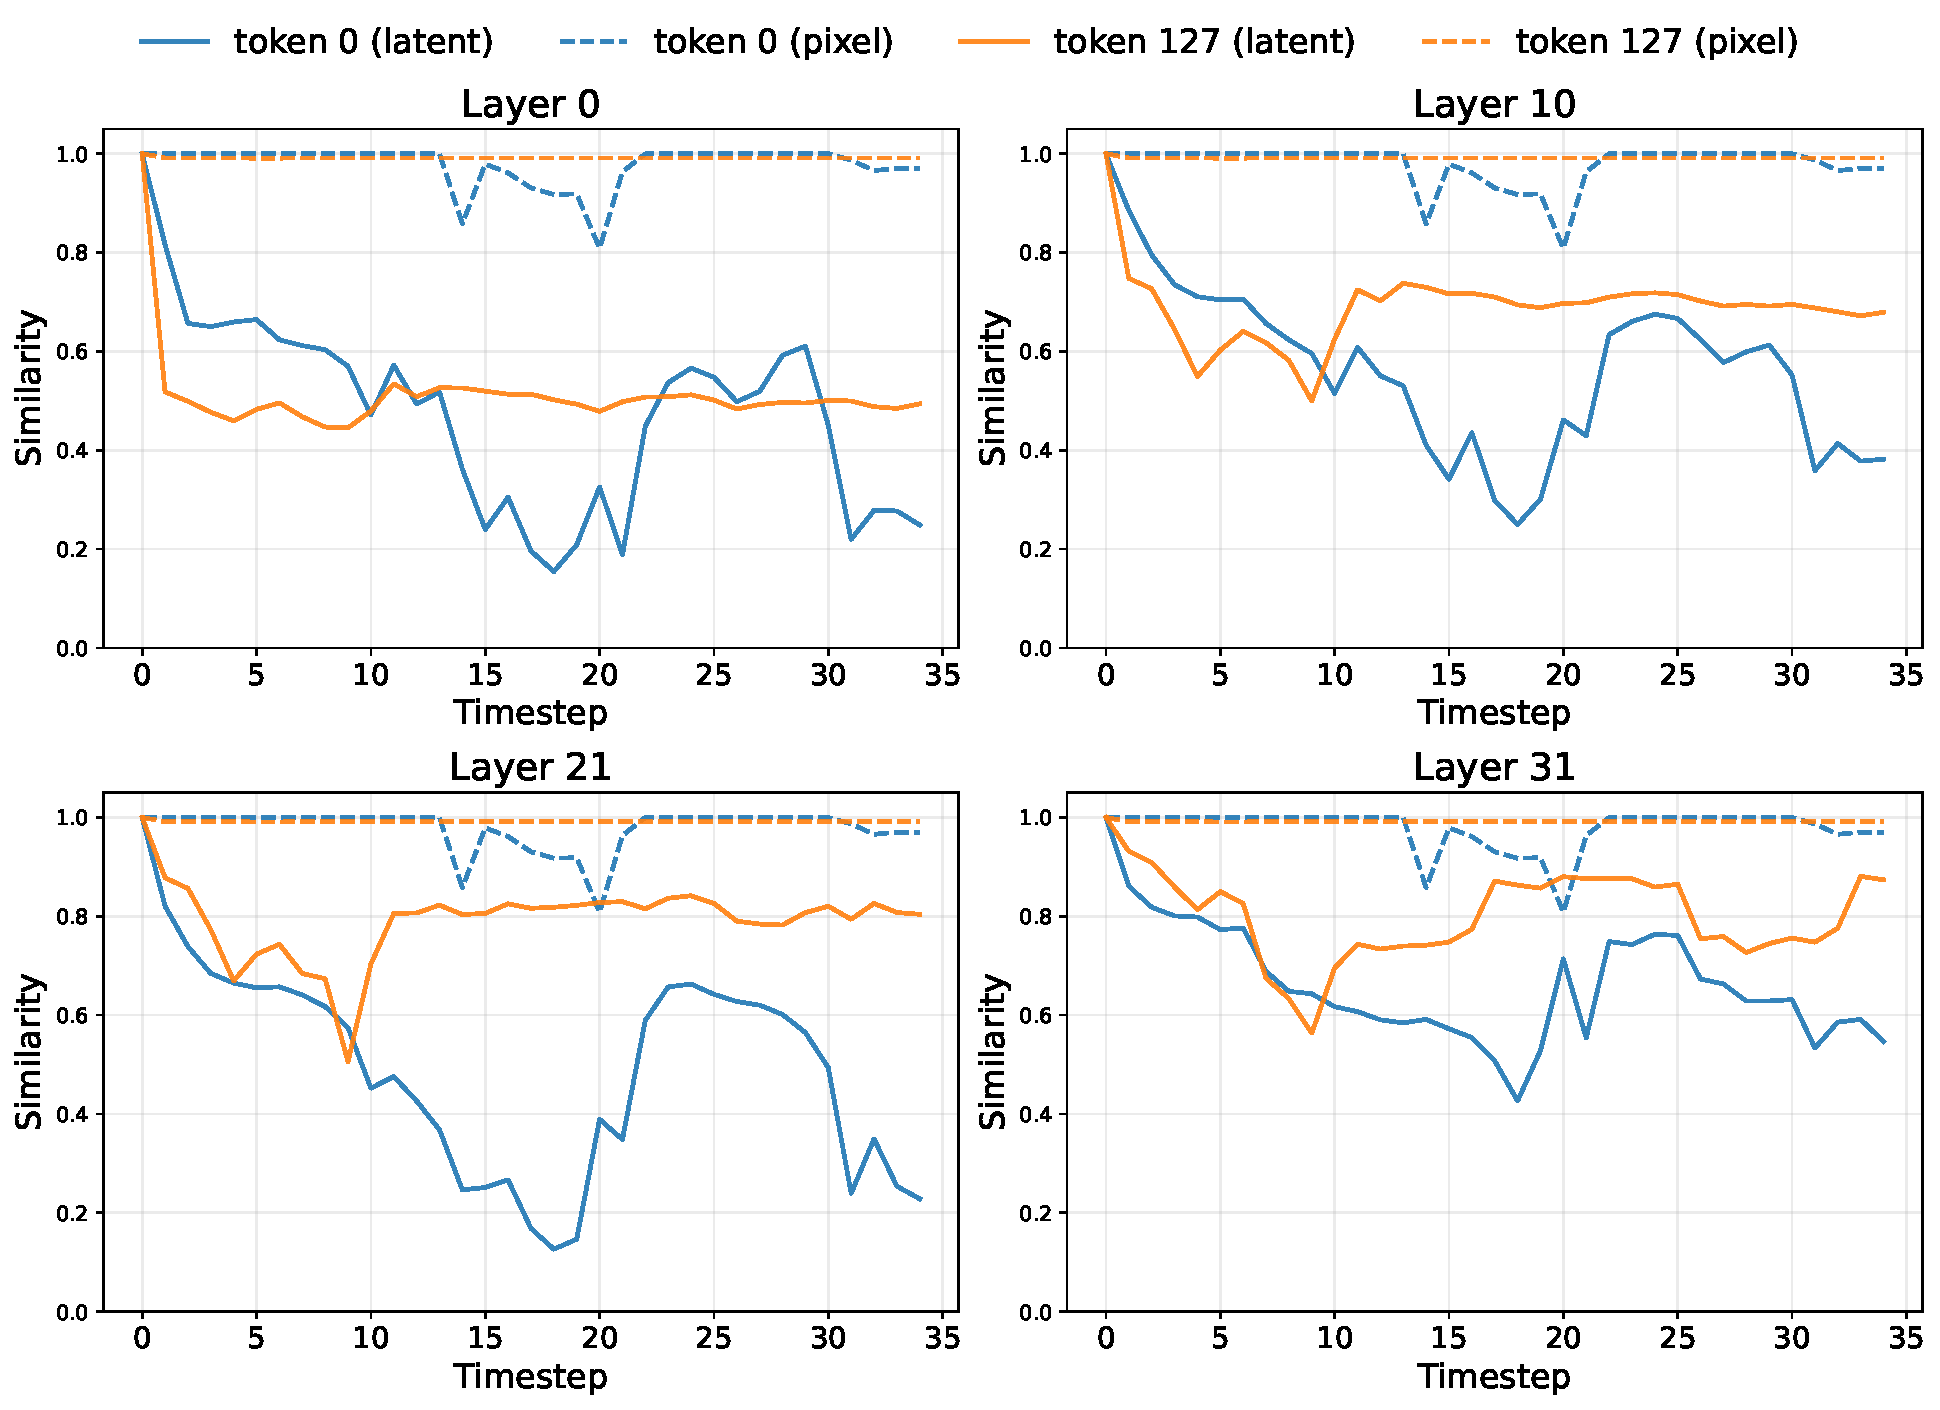
\includegraphics[width=1.0\linewidth]{figs/drift.pdf}
    \caption{Visually static regions in pixel space exhibit substantial latent representation drift across timesteps. }
    \label{fig:drift}
\end{figure}


\section{Latency Distribution}
\label{app:lat_dist}
We provide the latency distribution during rollout across tasks in Figure~\ref{fig:latency}. On the *Pick Can* task, ~86.0\% of steps fully reuse static tokens across all levels, resulting in low latency (~250 ms). A smaller fraction (~7.4\%) triggers an L2 refresh (~500 ms), while only 6.6\% of steps require an L1 refresh, leading to higher latency (~900 ms).

These results show that high-latency events are infrequent, with the vast majority of steps operating in the efficient reuse regime. Since our goal is to optimize overall rollout efficiency (in addition to enabling multi-frame integration), occasional latency spikes have a negligible impact on end-to-end performance.


\begin{figure}
    \centering
    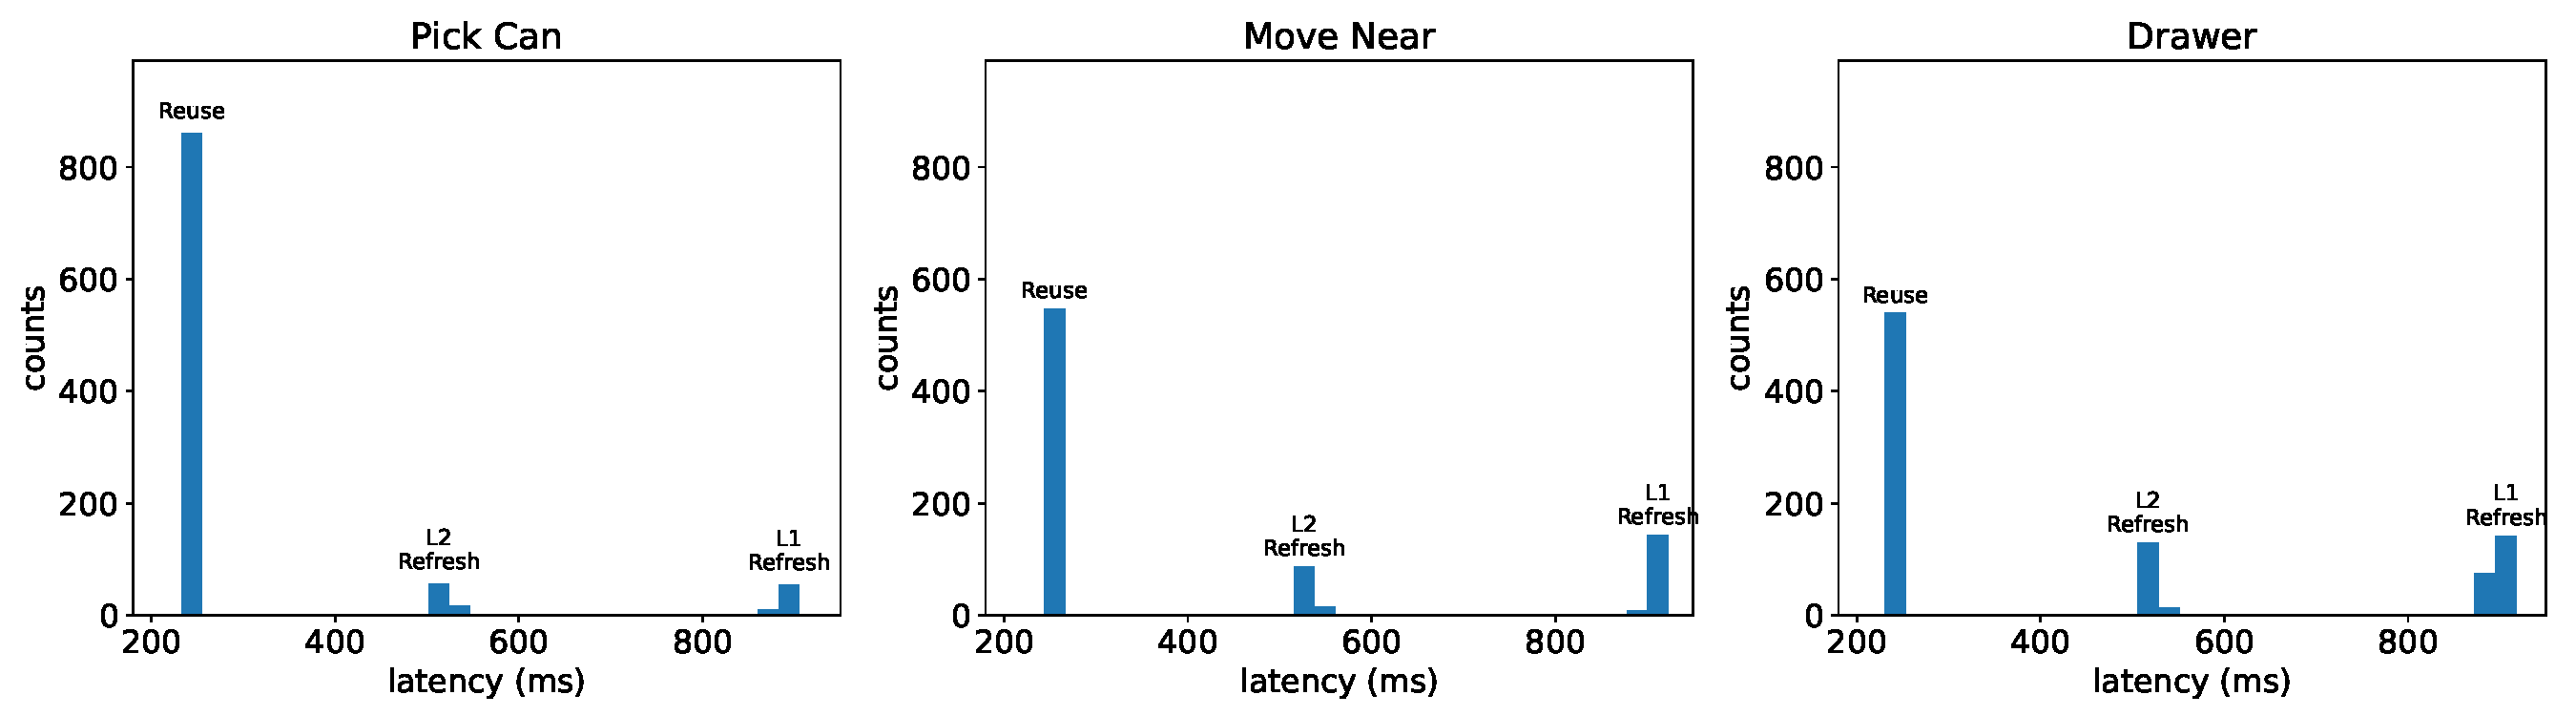
\includegraphics[width=1.0\linewidth]{figs/latency.pdf}
    \caption{The latency distribution for each step in rollouts. \emph{Reuse} means no refresh needed. \emph{Ln Refresh} means the need to refresh the n-th level static cache.}
    \label{fig:latency}
\end{figure}


\section{Hyperparameter Sensitivity}
In this section, we analyze the sensitivity of crucial hyperparameters.

\begin{figure}
    \centering
    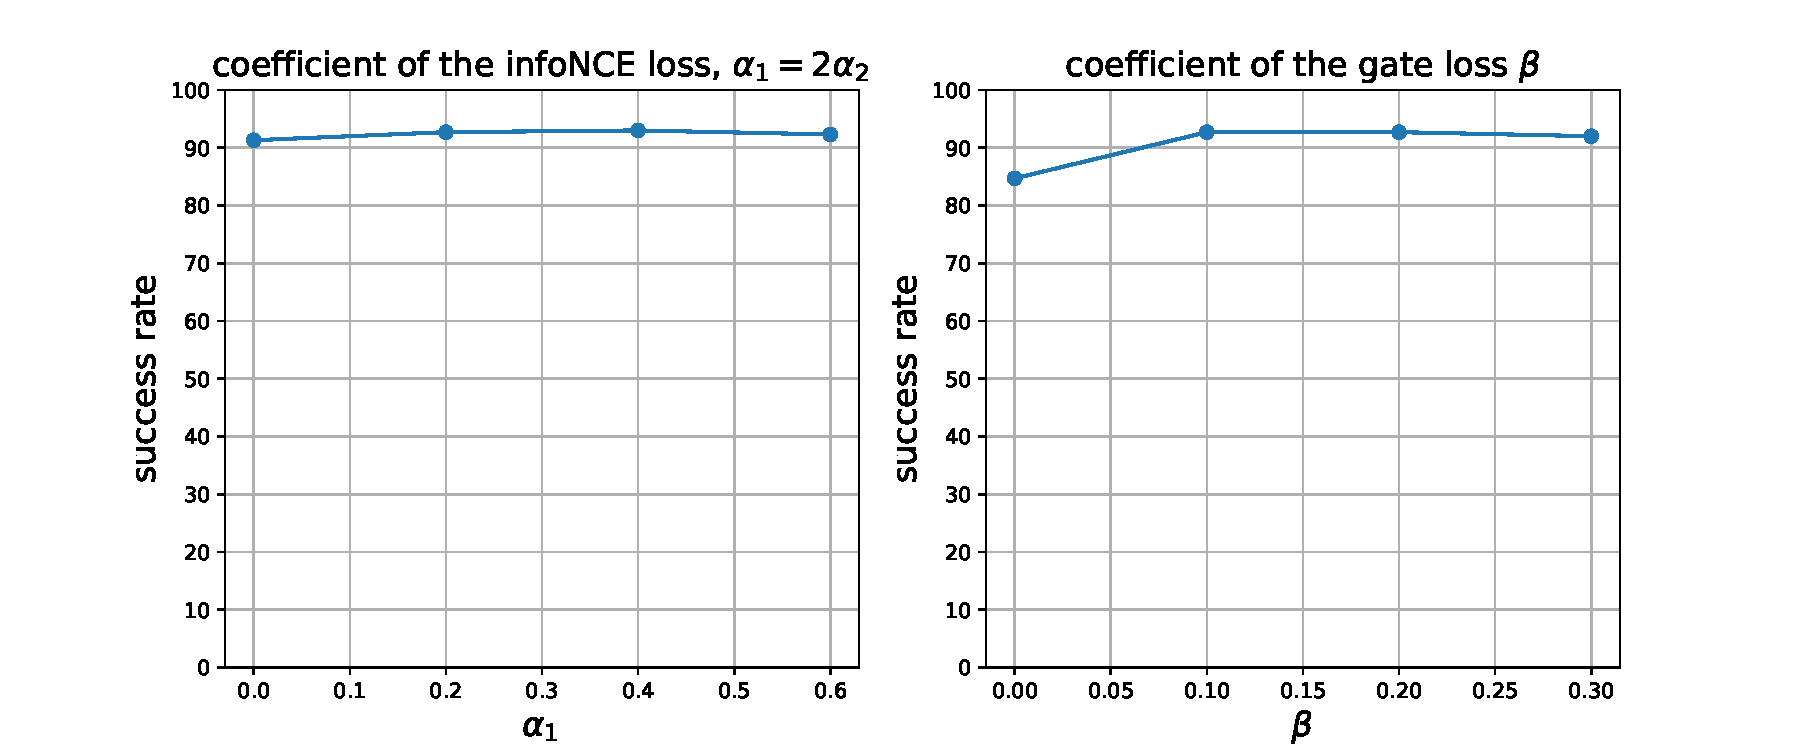
\includegraphics[width=0.8\linewidth]{figs/sensitivity.pdf}
    \caption{Sensitivity analysis on the coefficients for each loss term. Experiments are conducted on Pick Can (Visual Matching). }
    \label{fig:sensitivity}
\end{figure}

\subsection{Objective Coefficients}
\label{app:sense}

We conduct sensitivity analysis of important hyperparameters in our training objective, i.e., $\alpha$ and $\beta$ in our loss term. The results are plotted in Figure~\ref{fig:sensitivity}. 

For the coefficient $\alpha$ of $\mathcal{L}_\text{infoNCE}$, we find the performance to be stable across a broad range of values.

For the coefficient $\beta$ of $\mathcal{L}_\text{gate}$, we observe that performance is stable once $\beta \geq 0.1$. When $\beta = 0$, the recache gate is not effectively trained and degenerates to random refresh/reuse decisions, leading to significantly degraded performance.

\subsection{Static Ratio}
\label{app:static_ratio}
We consider the static ratio as a tunable hyperparameter that can be adapted to different environments. For more dynamic settings, it can be adjusted by (1) reducing the ratio during training to allocate more capacity to dynamic tokens, or (2) lowering the recache threshold for more frequent cache refreshing at test time.

Our sensitivity analysis in Figure~\ref{fig:static} shows stable performance across a broad range of ratios, with degradation only at extreme values.

\begin{figure}
    \centering
    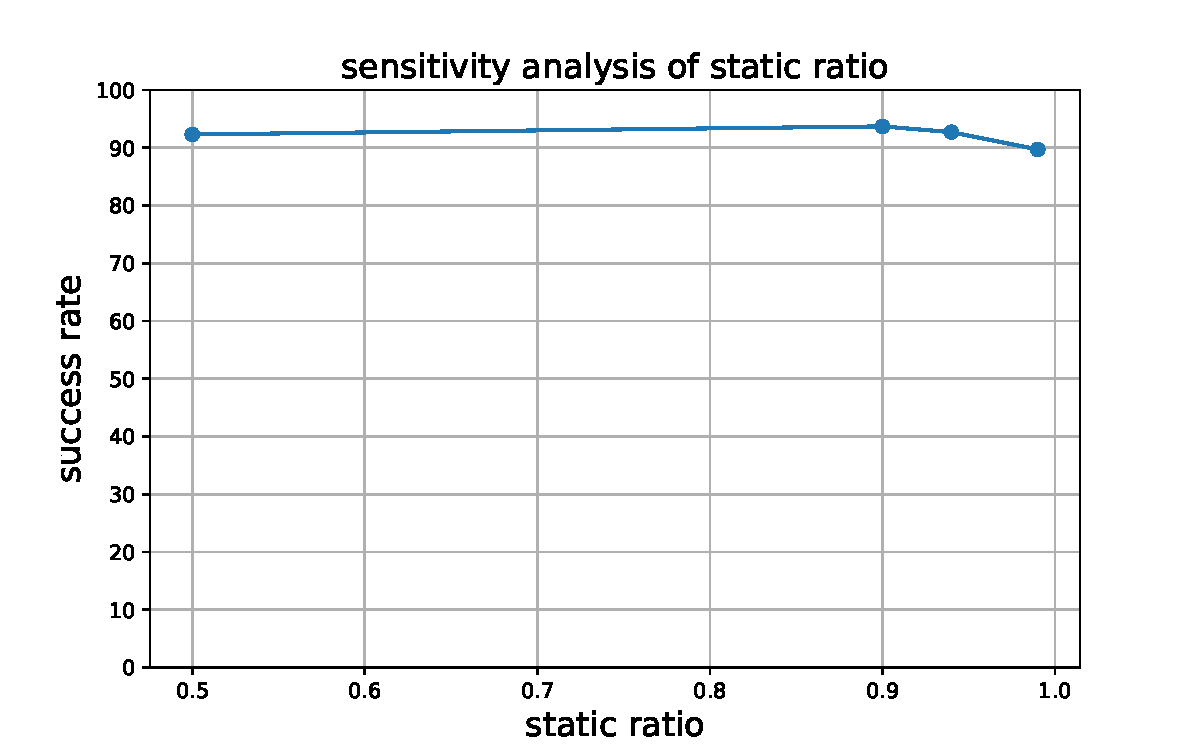
\includegraphics[width=0.5\linewidth]{figs/static.pdf}
    \caption{Sensitivity analysis of the static ratio. Experiments are conducted on Pick Can (Visual Matching).}
    \label{fig:static}
\end{figure}

% \begin{table}[]
%     \centering
%     \caption{Success rate (\%) on wrist image. Our model still achieves acceleration without the sacrifice of performance.}
%     \label{tab:real}
%     \begin{tabular}{l|c|c}
%     \toprule
%     Method & LIBERO-10 (wrist) & FLOPs \\
%     \midrule
%         OpenVLA-OFT &  $88.8$ & $100.0\%$ \\
%         + SD-VLA & $\mathbf{89.0}$ & $\mathbf{72.3\%}$\\
%     \bottomrule
%     \end{tabular}
% \end{table}


% \begin{table}[]
%     \centering
%     \caption{Success rate (\%) on LIBERO benchmark with $\pi_{0.5}$ \cite{intelligence2025pi05visionlanguageactionmodelopenworld}.}
%     \label{tab:real}
%     \begin{tabular}{l|cc|c}
%     \toprule
%     Method & Long & Spatial & FLOPs \\
%     \midrule
%         $\pi_{0.5}$ & $94.0\%$ & $96.8\%$ & $100.0\%$ \\
%         + SD-VLA & $\mathbf{94.2}\%$ & $\mathbf{97.8\%}$ & $\mathbf{48.9\%}$\\
%     \bottomrule
%     \end{tabular}
% \end{table}

\section{Temporal Evolution of Static-Dynamic Assignments}
\label{app:time_evo}

Below, we show a representative trajectory illustrating how \dysta{} adapts its static-dynamic assignments over time. As shown in Figure~\ref{fig:correctify}, the Pepsi can is initially treated as static because it is not intended to be manipulated. However, when unexpected contact occurs, the model detects the resulting change and reclassifies the can as dynamic, thereby triggering a cache refresh. In some cases, objects such as the orange may be treated as dynamic even though they remain unchanged. This does not affect task correctness, but only introduces a small amount of additional computational overhead.

\begin{figure}
    \centering
    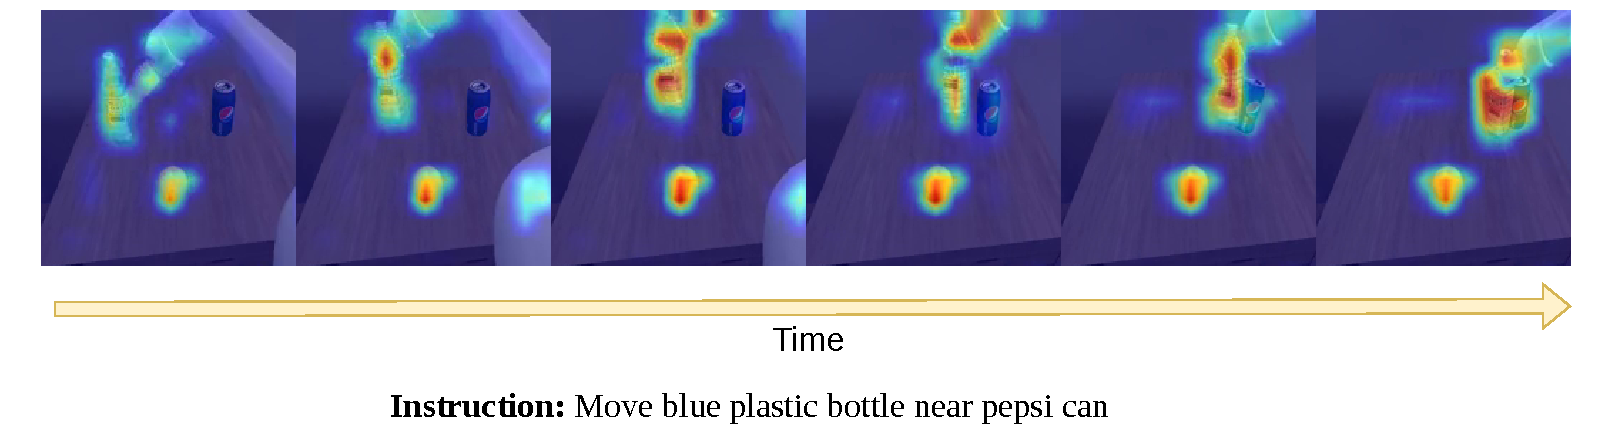
\includegraphics[width=\linewidth]{figs/rectify.pdf}
    \caption{An illustration that the model misclassifies objects and later corrects such errors.}
    \label{fig:correctify}
\end{figure}


% \begin{figure}
%     \centering
%     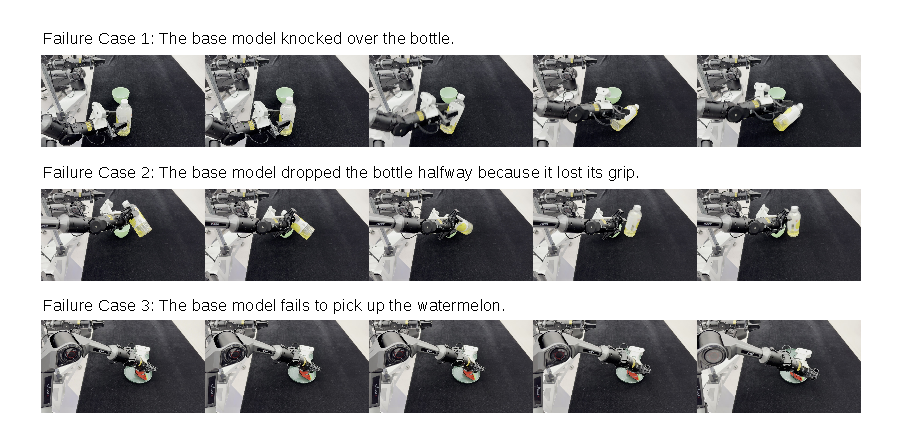
\includegraphics[width=\linewidth]{figs/fail.pdf}
%     \caption{Real-world failure cases of the VLA base model (OpenVLA-OFT \cite{kim2025fine})}
%     \label{fig:fail}
% \end{figure}

\section{Impact Statement}
This paper presents work whose goal is to advance the field of Machine Learning. There are many potential societal consequences of our work, none of which we feel must be specifically highlighted here.

\section{Declaration of LLM Usage}
We used large language models solely for editing and polishing the manuscript (e.g., grammar, phrasing, and typo correction). LLMs were not involved in the research ideation, methodology, experiments, or analysis, and do not constitute any original or non-standard component of this work.